\documentclass[10pt, aspectratio=169]{beamer} %
\usetheme{Singapore}

\usepackage{bookmark}
\usepackage{graphicx}
\usepackage[english]{babel}
\usepackage[utf8]{inputenc}
\usepackage[T1]{fontenc}
\usepackage{amsmath}
\usepackage{color}
\usepackage{listings}
\usepackage{tabularx}
\usepackage{amssymb}
\usepackage{lmodern}

\usepackage{hyperref}
\hypersetup{colorlinks=true, urlcolor=blue}

\DeclareMathOperator*{\minimize}{minimize} %in preamble
 
\newcommand{\N}{{\mathbb{N}}}
\newcommand{\I}{{\bf I}}
\newcommand{\C}{{\bf C}}
\newcommand{\A}{{\bf A}}
\newcommand{\T}{{\bf T}}
\newcommand{\g}{{\bf g}}
\newcommand{\e}{{\bf e}}
\newcommand{\ab}{{\bf a}}
\newcommand{\ba}{{\bf b}}
\newcommand{\Z}{{\mathbb{Z}}}
\newcommand{\R}{{\mathbb{R}}}
\newcommand{\mbf}{\mathbf}
\newcommand{\bs}{\boldsymbol}
\newcommand{\cc}{{\bf c}}
\newcommand{\su}{{\sum_{n=0}^{N-1}}}

\newcommand{\argmax}{\mathop{\text{arg\;max}}}
\newcommand{\argmin}{\mathop{\text{arg\;min}}}

\newcommand{\HH}{{\bf H}}
\newcommand{\thb}{\boldsymbol{\theta}}
\newcommand{\w}{{\bf w}}
\newcommand{\Sigb}{\boldsymbol{\Sigma}}
\newcommand{\mub}{\boldsymbol{\mu}}
\newcommand{\alb}{\boldsymbol{\alpha}}

\newcommand{\s}{{\bf s}}
\newcommand{\SB}{{\bf S}}

\definecolor{blue}{RGB}{32,32,255}
\graphicspath{{./images/}}

\newcommand{\h}{{\bf h}}
\newcommand{\rr}{{\bf r}}
\newcommand{\X}{{\bf X}}
\newcommand{\x}{{\bf x}}
\newcommand{\y}{{\bf y}}
\newcommand{\p}{{\bf p}}
\newcommand{\E}{{\bf E}}
\newcommand{\U}{{\bf U}}
\newcommand{\V}{{\bf V}}
\newcommand{\f}{{\bf f}}
\newcommand{\var}{{\mathop{\text{var}}}}

\newcommand{\F}{{\cal F}}
\newcommand{\leveys}{0.75\textwidth}
\newcommand{\etaisyys}{0.25\textwidth}

\newcommand{\sinc}{\mathop{\text{sinc}}}
\newcommand{\esim}{\em}

\newcommand{\modulo}{\operatorname{mod}}

\setbeamertemplate{frametitle continuation}[from second] 

\renewcommand{\insertcontinuationtext}{}

\setbeamertemplate{frametitle}
{
	\vspace*{0.7cm} \vbox{\insertframetitle}
}

\usecolortheme{default}

\setbeamertemplate{mini frames}{}
\renewcommand*{\slideentry}[6]{}
\setbeamertemplate{frametitle}{
    \vspace*{0.2cm}
    \insertframetitle
}

\title{Pattern Recognition and Machine Learning}
\subtitle{Slide Set 1: Introduction and the Basics of Python}
\author{Heikki Huttunen\\
heikki.huttunen@tut.fi}
\institute{Laboratory of Signal Processing\\Tampere University of Technology}
\date{January 2017}

\begin{document}

\maketitle

\lstdefinestyle{mystyle}{
  belowcaptionskip=1\baselineskip,
  breaklines=true,
  frame=single,
  xleftmargin=\parindent,
  language=Python,
  showstringspaces=false,
  basicstyle=\tiny\ttfamily,
  keywordstyle=\bfseries\color{green!40!black},
  commentstyle=\itshape\color{purple!40!black},
  identifierstyle=\color{blue},
  stringstyle=\color{orange},
  moredelim=**[is][\color{red}]{@}{@},
}

\lstset{language=Python,style=mystyle} 


\begin{frame}[allowframebreaks=0.8]
 {Course Organization}
\begin{itemize}

\item Organized on 3rd period; January -- February 2017.
\item Lectures every Tuesday 14-16 (TB111) and Friday 14-16 (TB111).
\item 9 groups of exercises between Tuesday and Friday (sign up at POP).
\item More details: \url{http://www.cs.tut.fi/courses/SGN-41007/}
\end{itemize}
\end{frame}

\begin{frame}[allowframebreaks=0.8]
 {Course Requirements}
\begin{enumerate}
\item 60\% of exercise assignments solved. For 70 \%, you get 1 point added to exam score;
for 80 \% two points and for 90\% three points. 
\item Project assignment, which is organized in the form of a pattern recognition competition. 
The competition is done in groups. \url{https://inclass.kaggle.com/c/gene-expression-prediction}
\item Written exam. Max. number of points for the exam is 30
with the following scoring.
\begin{center}
	\begin{tabular}{|| l || c | c | c | c | c | c ||}
	\hline\hline
	Points & <15 & <18 & <21 & <24 & <27 & $\ge$27 \\
	\hline
	Grade & 0 & 1 & 2 & 3 & 4 & 5 \\
	\hline\hline
	\end{tabular}
\end{center}

\end{enumerate}
\end{frame}

\begin{frame}[allowframebreaks=0.8]
 {Course Contents}
\begin{enumerate}
\item \textbf{Python:} Rapidly becoming the default platform for practical machine learning
\item \textbf{Estimation of Signal Parameters:} What are the phase, amplitude and frequency of this noisy sinusoid
\item \textbf{Detection Theory:} Detect whether there is a specific signal present or not
\item \textbf{Performance evaluation:} Cross-Validation, Bootstrapping, Receiver Operating Characteristics, other Error Metrics
\item \textbf{Machine Learning Models:} Logistic Regression, Support Vector Machine, Random Forests, Deep Learning
\item \textbf{Avoid Overlearning and Solve Ill-Posed Problems:} Regularization Techniques
\end{enumerate}
\end{frame}

\begin{frame}{Introduction}
    \begin{columns}
    \column{.7\textwidth} 
\begin{itemize}
\item Machine learning has become an important tool for multitude of scientific disciplines.
\item Training based approaches are rapidly substituting traditional
manually engineered pipelines.
\item \textbf{Training based} = we show examples of what is interesting
and hope the machine learns to do it for us
\item \textbf{Model based} = we have derived a model of the data and wish to
learn the unknown parameters
\item A few modern research topics:
\begin{itemize}
\item Image recognition (what is in this image and where?)
\item Speech recognition (what do I say?)
\item Medicine (data-driven diagnosis)
\end{itemize}
\end{itemize}
 \column{.3\textwidth}
\vspace*{-0.8cm}
\hspace*{-0.4cm}
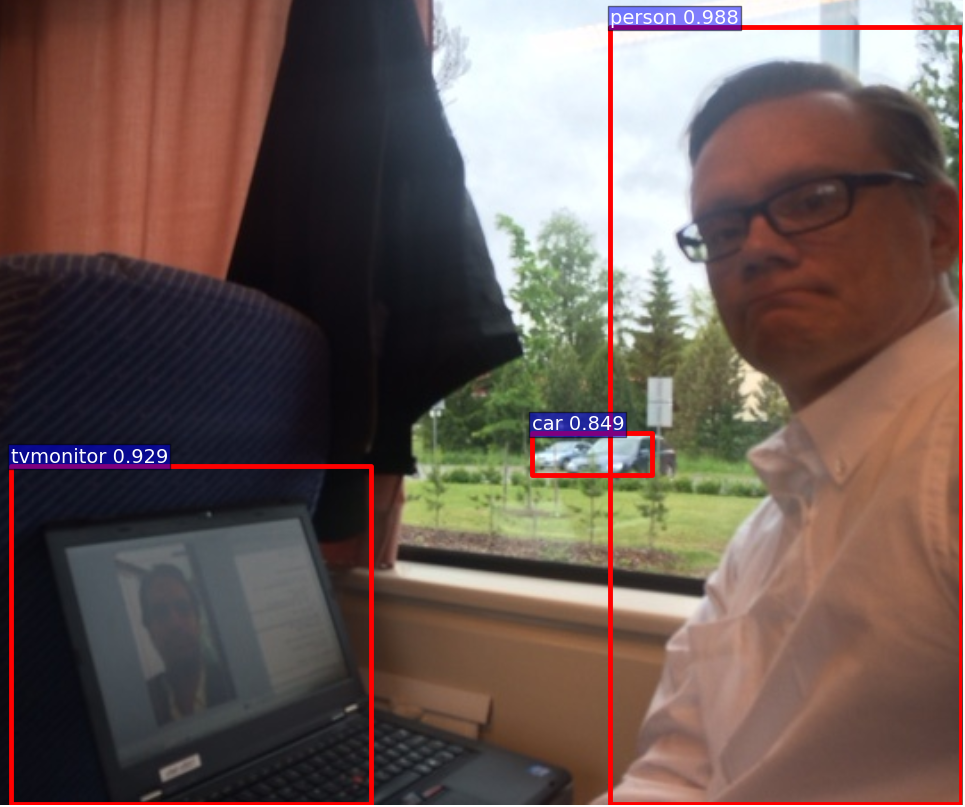
\includegraphics[width=1.2\columnwidth]{detections_hehu.png}\\
\vspace*{0.3cm}
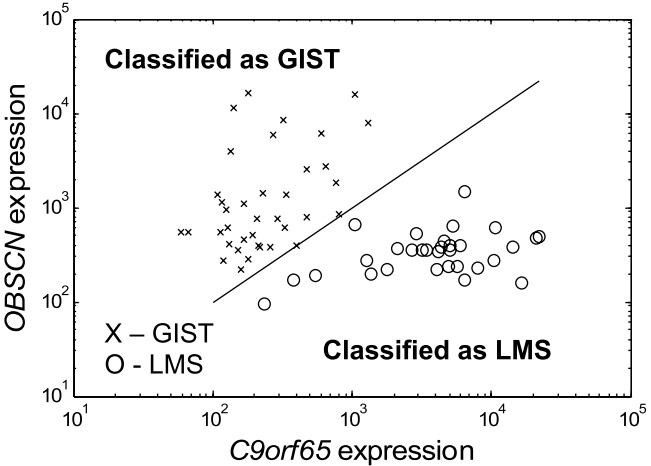
\includegraphics[width=\columnwidth]{Gist_Classification.png}\\
{\tiny \textbf{Price et al.}, "Highly accurate two-gene classifier for differentiating gastrointestinal stromal tumors and leiomyosarcomas," \emph{PNAS 2007}.\par}
\end{columns}
\end{frame}

\begin{frame}{Why Python?}
\begin{columns}
\column{0.65\textwidth}
\begin{itemize}
\item Python is becoming increasingly central tool for data science.
\item This was not always the case: 10 years ago everyone was using Matlab.
\item However, due to licensing issues and heavy development of Python,
scientific Python started to gain its user base.
\item Python's strength is in its variability and huge community. 
\item There are 2 versions: Python 2.7 and 3.6. We'll use the former one
as it's better supported by most packages interesting to us.
\end{itemize}
\column{0.35\textwidth}
\fbox{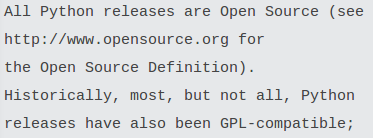
\includegraphics[width=1\columnwidth]{PythonLicense.png}}\\
\vspace*{0.1cm}
\fbox{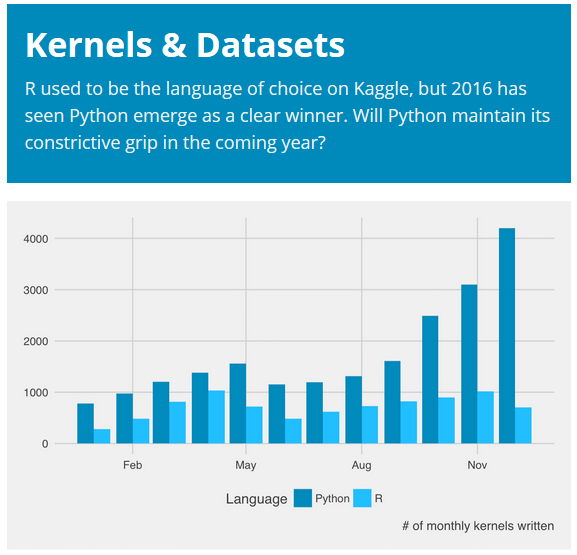
\includegraphics[width=\columnwidth]{py_vs_R.png}
}
\emph{\tiny Source: Kaggle.com newsletter, Dec. 2016}
\end{columns}
\end{frame}

\begin{frame}{Alternatives to Python in Science}
\begin{tabularx}{1.1\textwidth}{ l || l }

\textbf{Python vs. Matlab} & \textbf{Python vs. R} \\
\hline\hline
\begin{minipage}{0.48\textwidth}
{\small
\begin{itemize}
\item Matlab is \#1 workhorse for linear algebra.
\item Matlab is professionally maintained \emph{product}.
\item Some Matlab's toolboxes are great (Image Processing tb). 
Some are obsolete (Neural Network tb).
\item New versions twice a year. Amount of novelty varies.
\item Matlab is expensive for non-educational users.
\end{itemize}
}
\end{minipage}
&
\begin{minipage}{0.5\textwidth}
{\small
\begin{itemize}
\item R has been \#1 workhorse for statistics and data analysis. \footnote{\url{http://tinyurl.com/jynezuq}}
\item R is great for specific data analysis and visualization needs.
\item Lots of statistics community code in R.
\item Python interfaces with other domains ranging from deep neural networks (Caffe, Theano)
and image analysis (OpenCV) to even a fullblown webserver (Django/Flask)
\end{itemize}
}
\end{minipage}\\

\hline\hline
\end{tabularx}

\begin{itemize}
\item "Matlab is made for mathematicians, R for statisticians and Python for programmers."
\end{itemize}

\end{frame}

\begin{frame}{Essential Modules}
\begin{itemize}
\item \textbf{\href{http://www.numpy.org/}{numpy}}: The matrix / numerical analysis layer at the bottom
\item \textbf{\href{https://www.scipy.org/}{scipy}}: Scientific computing utilities (linalg, FFT, signal/image processing...)
\item \textbf{\href{http://scikit-learn.org}{scikit-learn}}: Machine learning (our focus here)
\item \textbf{\href{http://matplotlib.org/}{matplotlib}}: Plotting and visualization
\item \textbf{opencv}: Computer vision
\item \textbf{pandas}: Data analysis
\item \textbf{statsmodels}: Statistics in Python
\item \textbf{caffe, theano, tensorflow, \href{http://keras.io/}{keras}}: Deep neural networks (we are using keras later in the course)
\item \textbf{spyder}: The front end (Scientific PYthon Development EnviRonment)
\end{itemize}
\end{frame}


\begin{frame}{Where to get Python?}
\begin{itemize}
\item It is possible to construct your custom Python environment by installing
individual modules (base from \url{python.org} and libraries from, e.g.,
\url{http://www.lfd.uci.edu/~gohlke/pythonlibs/}).
\item Alternatively, one may install a full distribution, such as
\begin{itemize}
\item Anaconda \url{https://www.continuum.io/downloads} \textbf{$\leftarrow$ my favorite}
\item Enthought Canopy \url{http://www.enthought.com/}
\end{itemize}
\item ...or in linux:\\
\noindent\texttt{
\noindent\hspace*{0.8cm}\# apt-get install python\\
\hspace*{1cm}\# apt-get install python-numpy\\
\hspace*{1cm}\# apt-get install python-sklearn\\ 
\hspace*{1cm}\# apt-get install python-matplotlib\\
\hspace*{1cm}\# apt-get install spyder
}
\end{itemize}
\end{frame}

\begin{frame}[fragile]{The Language}
\begin{columns}
\column{0.65\textwidth}
{\small
\vspace*{-0.5cm}
\begin{itemize}
\item Python was designed to be a highly readable language.
\item Python uses whitespace to delimit program blocks. First you hate it,
later you love it.
\item All used modules are imported using an \verb+import+ declaration.
\item The members of a module are referred using the dot: \verb+np.cos([1,2,3])+
\item Interpreted language. Also interactive with IPython extensions.
\end{itemize}
}
\column{0.35\textwidth}
\fbox{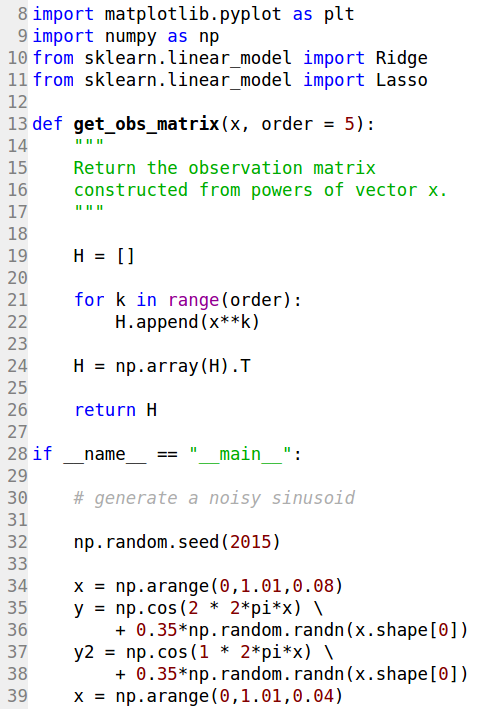
\includegraphics[width=1\columnwidth]{pythonExample.png}}
\end{columns}
\end{frame}

\begin{frame}[fragile]{Things to Come}
\begin{itemize}
\item Following slides will introduce the basic Python usage within scientific computing.
\begin{itemize}
\item \textbf{The editor and the environment} 
\begin{itemize}
\item \emph{Matlab slightly better than Python}
\end{itemize}
\item \textbf{Linear algebra} 
\begin{itemize}
\item \emph{Matlab better than Python}
\end{itemize}
\item \textbf{Programming constructs} (loops, classes, etc.) 
\begin{itemize}
\item  \emph{Python better than Matlab}
\end{itemize}
\item \textbf{Machine learning} 
\begin{itemize}
\item  \emph{Python a lot better than Matlab}
\end{itemize}
\end{itemize}
\end{itemize}
\end{frame}

\begin{frame}[fragile]{Spyder Editor}
\begin{columns}%[onlytextwidth]
\column{0.44\textwidth}
\begin{itemize}
\item In this course we use the \emph{Spyder} editor.
\item The editor window contains two panes: editor on the left and
console on the right.
\item \fbox{F5}: Run code; \fbox{F9}: Run selected region.
\item Alternatively, you can use whatever editor you like, and run
everything on the command line.
\end{itemize}
\column{0.55\textwidth}
\vspace*{-0.5cm}
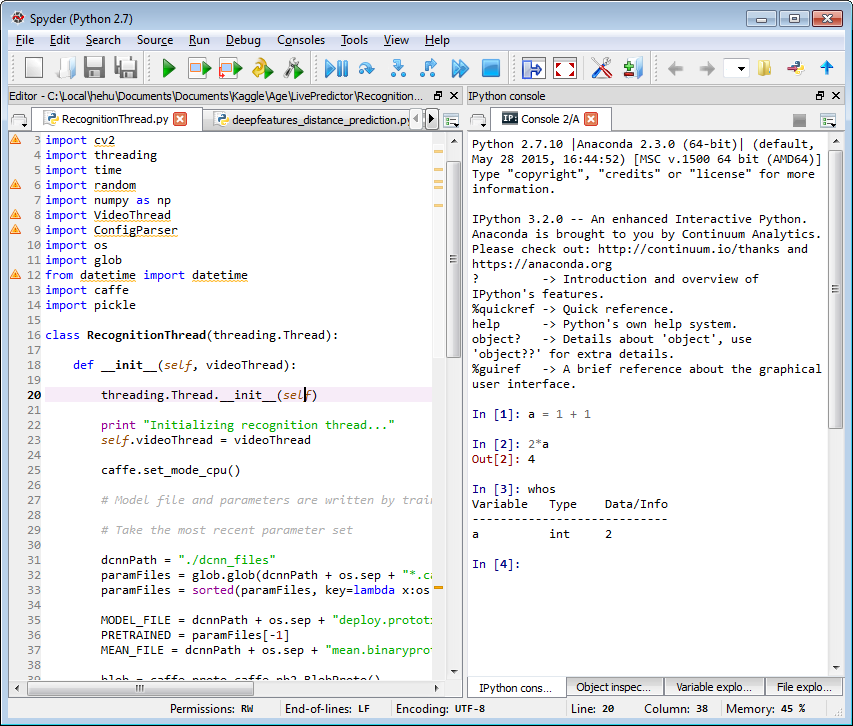
\includegraphics[width=1\columnwidth]{spyder.png}\\
\vspace*{0.2cm}
\centerline{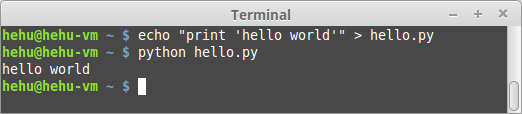
\includegraphics[width=0.8\columnwidth]{helloworld.png}}
\end{columns}
\end{frame}


\begin{frame}[fragile,allowframebreaks=0.8]
 {Python Basics}
\begin{columns}%[onlytextwidth]
\column{0.55\textwidth}
\begin{itemize}
\item Python code can be executed either from a script file (*.py) or in the
interactive mode (just like Matlab).
\item For the interactive mode; just execute \emph{python} from the command line.
\item Alternatively, \emph{ipython} (if installed) starts Python in a more
user-friendly mode:
\begin{itemize}
\item Tab-completion works
\item Many utility functions (\emph{e.g.,} \verb+ls+, \verb+pwd+, \verb+cd+)
\item \emph{Magic} functions (\emph{e.g.,} \verb+%run+, \verb+%timeit+, \verb+%edit+, \verb+%pastebin+)
\end{itemize}
\end{itemize}
\column{0.45\textwidth}
\vspace*{-0.5cm}
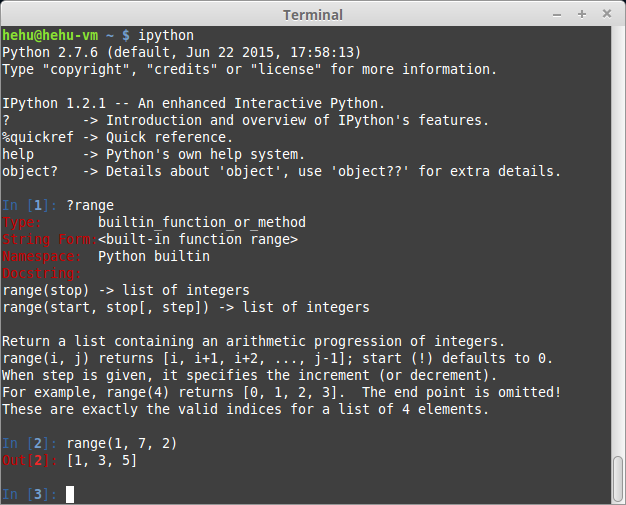
\includegraphics[width=1\columnwidth]{ipythonRange.png}\\
\vspace*{0.25cm}
{\small\it
Command
\verb+range+ creates a list of integers. Compare to Matlab's
syntax \verb+1:2:6+.
}
\end{columns}
\end{frame}

\begin{frame}[fragile,allowframebreaks=0.8]
 {Help}
\begin{itemize}
\item For each command, help is there to refresh your memory:
\begin{lstlisting}
>>> help("".strip) # strip is a member of the string class
Help on built-in function strip:

strip(...)
    S.strip([chars]) -> string or unicode
    
    Return a copy of the string S with leading and trailing
    whitespace removed.
    If chars is given and not None, remove characters in chars instead.
    If chars is unicode, S will be converted to unicode before stripping
\end{lstlisting}
\item In \emph{ipython}, the shortcut \verb+?+ is available, too (see previous slide).
\item Many people prefer to Google for \verb+python strip+ instead; matter of taste.
\end{itemize}
\end{frame}


\begin{frame}[fragile,allowframebreaks=0.8]
 {Using Modules}
\begin{columns}%[onlytextwidth]
\column{0.6\textwidth}
\begin{itemize}
\item Python libraries are called \emph{modules}.
\item Each module needs to be imported before use.
\item Three common alternatives:
\begin{enumerate}
	\item Import the full module: \verb+import numpy+
	\item Import selected functions from the module: \verb+from numpy import array, sin, cos+
	\item Import all functions from the module: \verb+from numpy import *+
\end{enumerate}
\end{itemize}

\column{0.4\textwidth}
\begin{lstlisting}
>>> sin(pi)

NameError: name 'sin' is not defined

>>> from numpy import sin, pi

>>> sin(pi)
1.2246467991473532e-16
\end{lstlisting}

\begin{lstlisting}
>>> import numpy as np

>>> np.sin(np.pi)
1.2246467991473532e-16
\end{lstlisting}

\begin{lstlisting}
>>> from numpy import *

>>> sin(pi)
1.2246467991473532e-16
\end{lstlisting}

\end{columns}
\end{frame}


\begin{frame}[fragile,allowframebreaks=0.8]
 {Using Modules}
\begin{columns}%[onlytextwidth]
\column{0.6\textwidth}
A few things to note:
\begin{itemize}
	\item All methods support shortcuts; \emph{e.g.,} \verb+import numpy as np+.
	\item Sometimes \verb+import <module>+ fails, if the module is in fact a collection of modules.
	For example, \verb+import scipy+. Instead, use \verb+import scipy.signal+
	\item Importing all functions from the module is not recommended, because different modules
	may contain functions with the same name.
\end{itemize}
\column{0.4\textwidth}
\begin{lstlisting}
>>> import scipy

>>> matfile = scipy.io.loadmat("myfile.mat")

AttributeError: 'module' object has no attribute 'io'
\end{lstlisting}
\begin{lstlisting}
>>> import scipy.io as sio

>>> matfile = sio.loadmat("myfile.mat") # Works OK
\end{lstlisting}
\begin{lstlisting}
>>> from scipy.io import loadmat

>>> matfile = loadmat("myfile.mat") # Works OK
\end{lstlisting}

\end{columns}
\end{frame}

\begin{frame}[fragile,allowframebreaks=0.8]
 {NumPy}
\begin{columns}%[onlytextwidth]
\column{0.6\textwidth}
\begin{itemize}
\item Practically all scientific computing in Python is based on \verb+numpy+ and \verb+scipy+ modules.
\item NumPy provides a numerical array as an alternative to Python list.
\item The list type is very generic and accepts any mixture of data types.
\item Although practical for generic manipulation, it is becomes inefficient in computing.
\item Instead, the NumPy array is more limited and more focused on numerical computing.
\end{itemize}
\column{0.4\textwidth}
\begin{lstlisting}
# Python list accepts any data types
v = [1, 2, 3, "hello", None]
\end{lstlisting}
\begin{lstlisting}
# We like to call numpy briefly "np"
>>> import numpy as np 

# Define a numpy array (vector):
>>> v = np.array([1, 2, 3, 4])

# Note: the above actually casts a 
# Python list into a numpy array.

# Resize into 2x2 matrix
>>> V = np.resize(v, (2, 2))

# Invert:
>>> np.linalg.inv(V)
array([[-2. ,  1. ],
       [ 1.5, -0.5]])
\end{lstlisting}

\end{columns}
\end{frame}

\begin{frame}[fragile,allowframebreaks=0.8]
 {More on Vectors}
\begin{itemize}
\item \verb+np.arange+ creates a range array (like \verb+1:0.5:10+ in Matlab)
\begin{lstlisting}
>>> np.arange(1, 10, 0.5) # Arguments: (start, end, step)
array([ 1. ,  1.5,  2. ,  2.5,  3. ,  3.5,  4. ,  4.5,  5. ,  5.5,  6. ,
        6.5,  7. ,  7.5,  8. ,  8.5,  9. ,  9.5])
				
# Note that the endpoint is not included (unlike Matlab).
\end{lstlisting}
\item Most vector/matrix functions are similar to Matlab:
\begin{lstlisting}
>>> np.linspace(1, 10, 5) # Arguments: (start, end, num_items)
array([  1.  ,   3.25,   5.5 ,   7.75,  10.  ])

>>> np.eye(3)
array([[ 1.,  0.,  0.],
       [ 0.,  1.,  0.],
       [ 0.,  0.,  1.]])
			
>>> np.random.randn(2, 3)
array([[-2.23506417,  0.47311746,  0.05343861],
       [ 1.255074  , -0.03576461,  0.96121907]])
\end{lstlisting}
\end{itemize}
\end{frame}


\begin{frame}[fragile,allowframebreaks=0.8]
 {Matrices}
\begin{itemize}
\item A matrix is defined similarly; either by specifying the values
manually, or using special functions.
\begin{lstlisting}
# A matrix is simply an array of arrays
# May seem complicated at first, but is in fact
# nice for N-D arrays.

>>> np.array([[1, 2], [3, 4]])
array([[1, 2],
       [3, 4]])

>>> from scipy.linalg import toeplitz, hilbert # You could also " ...import *"
>>> toeplitz([3, 1, -2])
array([[ 3,  1, -2],
       [ 1,  3,  1],
       [-2,  1,  3]])

>>> hilbert(3)
array([[ 1.        ,  0.5       ,  0.33333333],
       [ 0.5       ,  0.33333333,  0.25      ],
       [ 0.33333333,  0.25      ,  0.2       ]])
\end{lstlisting}
\end{itemize}
\end{frame}

\begin{frame}[fragile,allowframebreaks=0.8]
{Matrix Product}
\begin{columns}%[onlytextwidth]
\column{0.5\textwidth}
\begin{itemize}
\item Matrix multiplication is different from Matlab.
Use \verb+np.dot+ or \verb+np.matmul+.
\item With NumPy version 1.10+ and Python 3.5+, matrix multiplication can be done
with the \verb+@+ operator: \verb+A @ B+.
\end{itemize}
\column{0.5\textwidth}
\begin{lstlisting}
>>> A = np.array([[1, 2], [3, 4]])
>>> B = np.array([[5, 6], [7, 8]])

>>> A * B # Elementwise product (Matlab: A .* B)
array([[ 5, 12],
       [21, 32]])

>>> np.dot(A, B) # Matrix product; alternatively: np.matmul
array([[19, 22],
       [43, 50]])
\end{lstlisting}

\begin{lstlisting}[escapeinside={(*}{*)}]
$ python3
Python 3.5.2 (default, Nov 17 2016, 17:05:23) 
>>> import numpy as np
>>> A = np.random.rand(3,3)
>>> B = np.random.rand(3,3)
>>> A(* @ *)B
array([[ 0.28382296,  0.90172558,  1.10036663],
       [ 0.39959554,  1.12141386,  1.39473854],
       [ 0.28797509,  0.82918235,  1.04229714]])
\end{lstlisting}
\end{columns}
\end{frame}

\begin{frame}[fragile]
 {Indexing}
\begin{itemize}
\item Indexing of vectors uses the colon notation, too.
\item Below, we extract selected items from the vector \verb+1...10+:
\begin{lstlisting}
>>> x = np.arange(1, 11)
>>> x[0:8:2] # Unlike Matlab, indexing starts from 0
array([1, 3, 5, 7])

# Note: use square brackets for indexing
# Note2: colon operator has the order start:end:step;
# not start:step:end as in Matlab
\end{lstlisting}
\item The start and end points can be omitted:
\begin{lstlisting}
>>> x[5:] # All items from the 5'th
array([ 6,  7,  8,  9, 10])
>>> x[:5] # All items until the 5'th
array([1, 2, 3, 4, 5])
>>> x[::3] # All items with step 3
array([ 1,  4,  7, 10])
\end{lstlisting}
\end{itemize}
\end{frame}

\begin{frame}[fragile,allowframebreaks=0.8]
 {Indexing}
\begin{columns}
\column{0.6\textwidth}
\begin{itemize}
\item Negative indices are counted from the end\\ (-1 = the last, -2 = second-to-last, etc.):
\end{itemize}
\column{0.4\textwidth}
\begin{lstlisting}
>>> x[-3:] # Three last items
array([ 8,  9, 10])
>>> x[::-1] # Items in inverse order
array([10,  9,  8,  7,  6,  5,  4,  3,  2,  1])
\end{lstlisting}
\end{columns}
\centerline{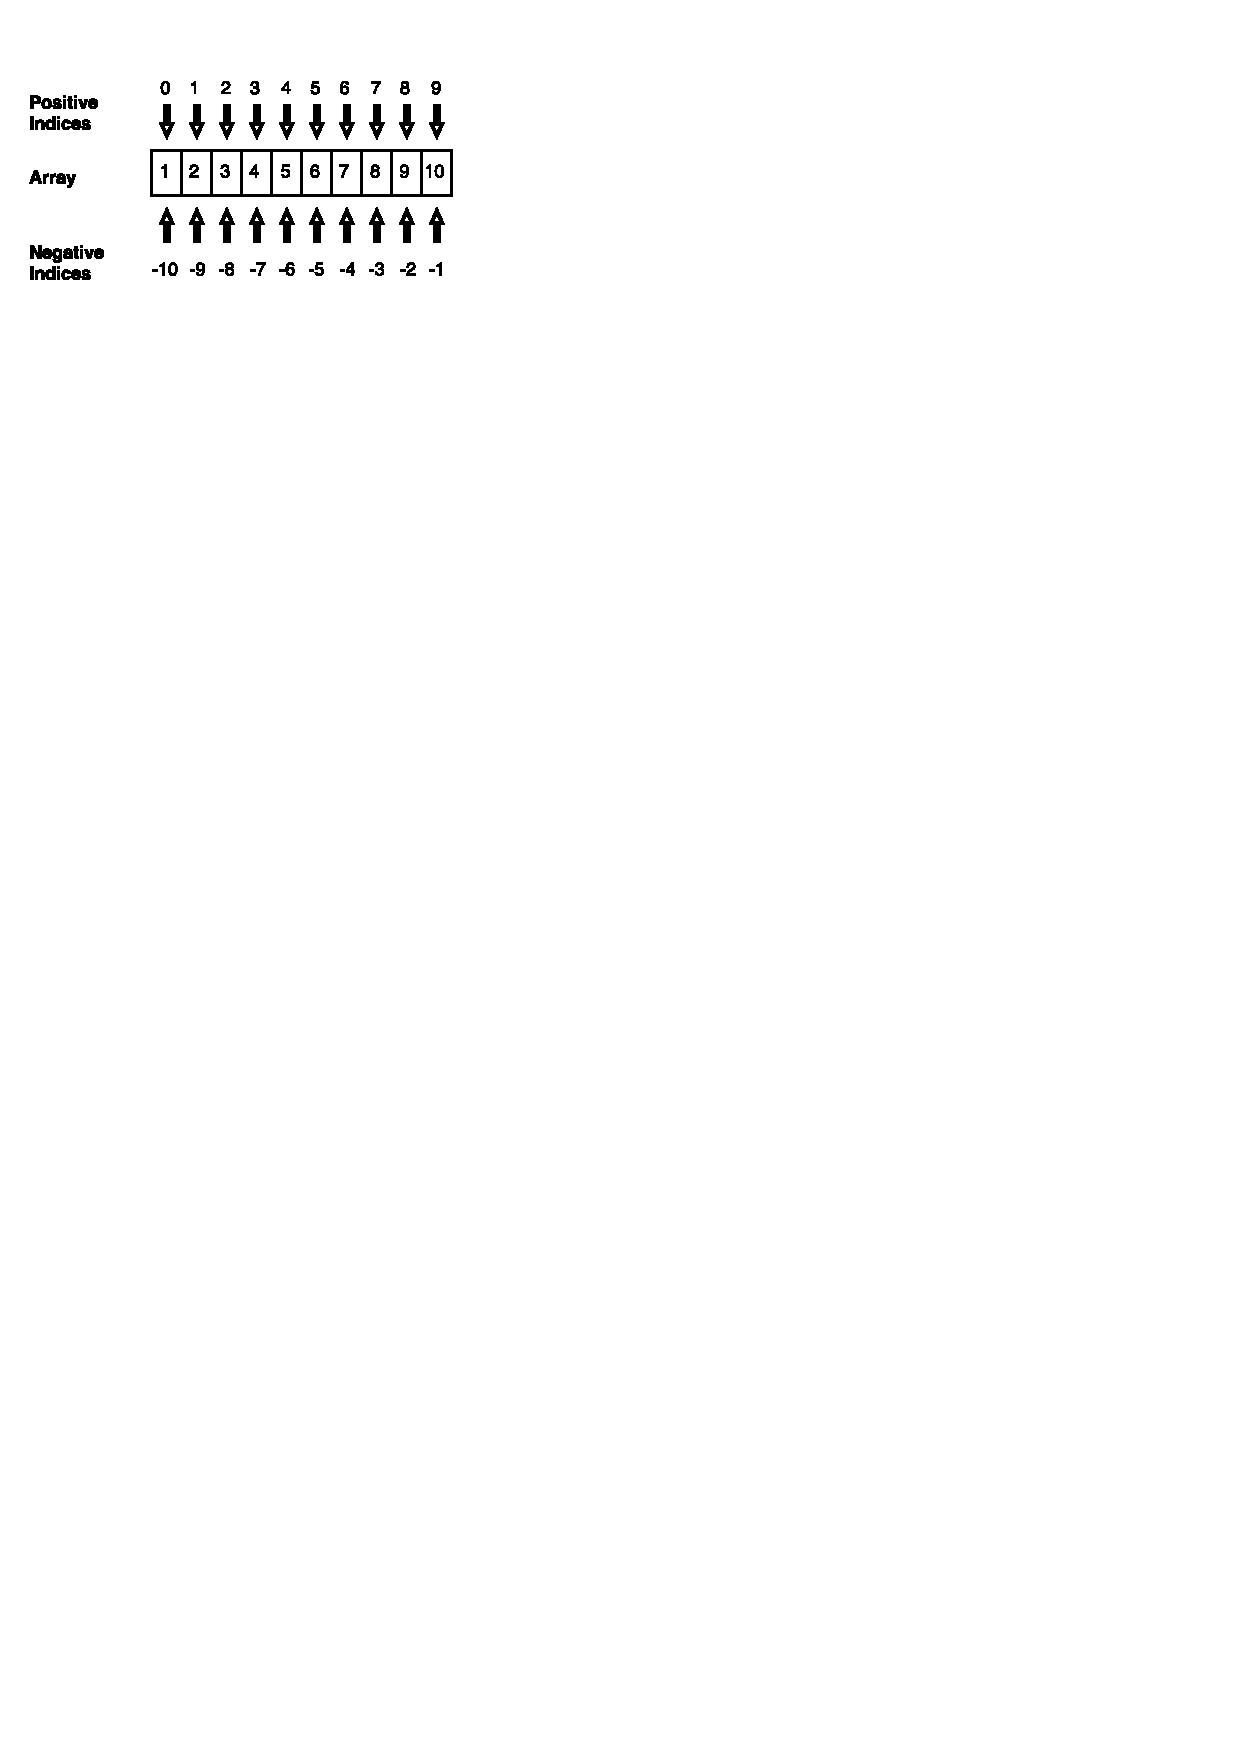
\includegraphics[width=0.45\textwidth]{Indexing.pdf}}
\end{frame}


\begin{frame}[fragile,allowframebreaks=0.8]
 {Indexing}
\begin{itemize}
\item Also matrices can be indexed similarly. This operation is called \emph{slicing},
and the result is a \emph{slice} of the matrix.
\end{itemize}
\vspace*{-0.2cm}
\begin{columns}
\hspace*{0.05cm}
\column{0.6\textwidth}
\begin{itemize}
\item Here we request for items on the rows 2:4~=~[2,3] and columns 1,2,4 (shown in red).
\item Note, that with matrices, the first index is the row; not "x-coordinate".
\item This order is called "Fortran style" or "column major" while the alternative is 
"C~style" or "row major".
\end{itemize}
\column{0.35\textwidth}
\begin{lstlisting}
>>> M = np.reshape(np.arange(0, 36), (6, 6))
array([[ 0,  1,  2,  3,  4,  5],
       [ 6,  7,  8,  9, 10, 11],
       [12, @13@, @14@, 15, @16@, 17],
       [18, @19@, @20@, 21, @22@, 23],
       [24, 25, 26, 27, 28, 29],
       [30, 31, 32, 33, 34, 35]])

>>> M[2:4, [1,2,4]]
array([[13, 14, 16],
       [19, 20, 22]])
\end{lstlisting}
\end{columns}
\end{frame}

\begin{frame}[fragile,allowframebreaks=0.8]
 {Indexing}
\begin{itemize}
\item To specify only column or row indices, use ":" alone.
\end{itemize}
\vspace*{-0.3cm}
\begin{columns}[T]
\hspace*{0.05cm}
\column{0.6\textwidth}
\begin{itemize}
\item Now we wish to extract two bottom rows.
\item \verb+M[4:, :]+ reads "give me all rows after the 4th and all columns".
\item In this case, alternative forms would be, \emph{e.g.,} \verb+M[-2:, :]+ and \verb+M[[4,5], :]+.
\end{itemize}
\column{0.35\textwidth}
\begin{lstlisting}
>>> M = np.reshape(np.arange(0, 36), (6, 6))
array([[ 0,  1,  2,  3,  4,  5],
       [ 6,  7,  8,  9, 10, 11],
       [12, 13, 14, 15, 16, 17],
       [18, 19, 20, 21, 22, 23],
       [@24@, @25@, @26@, @27@, @28@, @29@],
       [@30@, @31@, @32@, @33@, @34@, @35@]])

>>> M[4:, :]
array([[24, 25, 26, 27, 28, 29],
       [30, 31, 32, 33, 34, 35]])
\end{lstlisting}
\end{columns}
\end{frame}

\begin{frame}[fragile]
 {N-Dimensional arrays}
\begin{columns}
\column{0.65\textwidth}
\begin{itemize}
\item Higher-dimensional arrays are frequently encountered in machine learning.
\item For example, a set of 1000 color images of size $w\times h = 128\times96$ is represented
as a $1000\times 3 \times 96\times 128$ array.
\item Here, dimensions are: image index, color channel, y-coordinate, x-coordinate.
\item Sometimes, a shorter name is used: \mbox{"(b, c, 0, 1) order"}.
\end{itemize}
\column{0.35\textwidth}
\begin{lstlisting}
# Generate a random "image" array:
>>> A = np.random.rand(1000, 3, 96, 128)

# What size is it?
>>> A.shape
(1000L, 3L, 96L, 128L)

# Access the pixel (4, 3) of 2nd color channel 
# of the 2nd image
>>> A[1, 2, 3, 4]
0.36569219631994954

# Request all color channels:
>>> A[1, :, 3, 4]
array([ 0.32306666,  0.60012626,  0.3656922 ])

# Request a complete 96x128 color channel:
>>> A[1, 2, :, :]
array([[ 0.19102217 ...
 0.88464718]])

# Equivalent shorter notation:
>>> A[1, 2, ...]
array([[ 0.19102217 ...
 0.88464718]])
\end{lstlisting}
\end{columns}
\end{frame}

\begin{frame}[fragile,allowframebreaks=0.8]
 {Functions}
\begin{columns}[onlytextwidth]

\column{0.55\textwidth}
\begin{itemize}
\item Functions are defined using the \verb+def+ keyword.
\item Function definition can appear anywhere in the code.
\item Functions can be imported to other files using \verb+import+.
\item Function arguments can be \emph{positional} or \emph{named} (see code).
\item Named arguments improve readability and are handy for 
setting the last argument in a long list.
\end{itemize}
\column{0.35\textwidth}
\begin{lstlisting}
# Define our first function
def hello(target):
    print ("Hello " + target + "!")
		
>>> hello("world")
Hello world!

>>> hello("Finland")
Hello Finland!

# We can also define the default argument:
def hello(target = "world"):
    print ("Hello " + target + "!")

>>> hello()
Hello world!

>>> hello("Finland")
Hello Finland!

# One can also assign using the name:

>>> hello(target = "Finland")
Hello Finland!
\end{lstlisting}

\end{columns}
\end{frame}

\begin{frame}[fragile,allowframebreaks=0.8]
 {Loops and Stuff}
\begin{columns}[onlytextwidth]
\column{0.55\textwidth}
\begin{lstlisting}
for lang in ['Assembler', 'Python', "Matlab", 'C++']:
    if lang in ["Assembler", "C++"]:
        print ("I am ok with %s." % (lang))
    else:
        print ("I love %s." % (lang))
\end{lstlisting}
\begin{lstlisting}
I am ok with Assembler.
I love Python.
I love Matlab.
I am ok with C++.
\end{lstlisting}
\begin{lstlisting}
# Read all lines of a file until the end

fp = open("myfile.txt", "r")
lines = []

while True:
    
    try:
        line = fp.readline()
        lines.append(line)
    except:
        # File ended
        break

fp.close()
\end{lstlisting}
\column{0.45\textwidth}
\begin{itemize}
\item Loops and other usual programming constructs are easy to remember.
\item \verb+for+ can loop over anything \emph{iterable}, such as a list or a file.
\item In Matlab, appending values to a vector in a loop is not recommended.
Python lists are actual lists, so appending is fine.
\end{itemize}
\end{columns}
\end{frame}

\begin{frame}[fragile]
 {Example: Reading in a Data File}
\begin{columns}
\column{0.53\textwidth}
\begin{itemize}
\item Suppose we need to read a csv file (text file with Comma Separated Values) into Python.
\end{itemize}
\column{0.4\textwidth}
\fbox{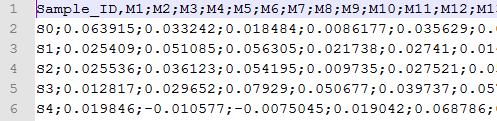
\includegraphics[width=\textwidth]{ovarian.png}}
\end{columns}
\begin{itemize}
\item The file consists of 216 rows (samples) with 4000 measurements each.
\item We will write file reading code from scratch.
\item Alternatively, many modules contain csv-reading functions
\begin{itemize}
\item \verb+numpy.loadtxt+ or \verb+numpy.genfromtxt+
\item \verb+csv.reader+
\item \verb+pandas.read_csv+
\end{itemize}
\end{itemize}
\end{frame}

\begin{frame}[fragile,allowframebreaks=0.8]{Example: Reading in a Data File}
\begin{columns}
\column{0.4\textwidth}
\begin{lstlisting}
import numpy as np

if __name__ == "__main__":

    X = [] # Rows of the file go here
    
    # We use Python's with statement. 
    # Then we do not have to worry 
    # about closing it.
    
    with open("ovarian.csv", "r") as fp:
        
        # File is iterable, so we can 
        # read it directly (instead of 
        # using readline).
        
        for line in fp:
            
            # Skip the first line:
            if "Sample_ID" in line:
                continue
\end{lstlisting}
\column{0.4\textwidth}
\begin{lstlisting}
            # Otherwise, split the line
            # to numbers:
            values = line.split(";")
            
            # Omit the first item 
            # ("S1" or similar):
            values = values[1:]
            
            # Cast each item from
            # string to float:
            values = [float(v) for v in values]

            # Append to X
            X.append(values)            
            
    # Now, X is a list of lists. Cast to 
    # Numpy array:
    X = np.array(X)
    
    print ("All data read.")
    print ("Result size is %s" % (str(X.shape)))
\end{lstlisting}
\end{columns}
\end{frame}


\begin{frame}[fragile,allowframebreaks=0.8]
 {Visualization}
\begin{columns}[onlytextwidth]
\column{0.35\textwidth}
\begin{lstlisting}
import matplotlib.pyplot as plt
import numpy as np

N = 100
n = np.arange(N) # Vector [0,1,2,...,N-1]
x = np.cos(2 * np.pi * n * 0.03)
x_noisy = x + 0.2 * np.random.randn(N)

fig = plt.figure(figsize = [10,5])

plt.plot(n, x, 'r-', 
         linewidth = 2, 
         label = "Clean Sinusoid")
				
plt.plot(n, x_noisy, 'bo-', 
         markerfacecolor = "green", 
         label = "Noisy Sinusoid")

plt.grid("on")
plt.xlabel("Time in $\mu$s")
plt.ylabel("Amplitude")
plt.title("An Example Plot")
plt.legend(loc = "upper left")

plt.show()
plt.savefig("../images/sinusoid.pdf", 
            bbox_inches = "tight")
\end{lstlisting}
\column{0.65\textwidth}
\begin{itemize}
\item The \texttt{matplotlib} module is our plotting library.
\item Function names are often similar to Matlab.
\item Usually you want to "\texttt{import~matplotlib.pyplot}".
\item Alternatively,
"\texttt{from matplotlib.pylab import *}" makes the environment very similar to Matlab.
\item Code also in \url{https://github.com/mahehu/SGN-41007}
\end{itemize}
\begin{center}
	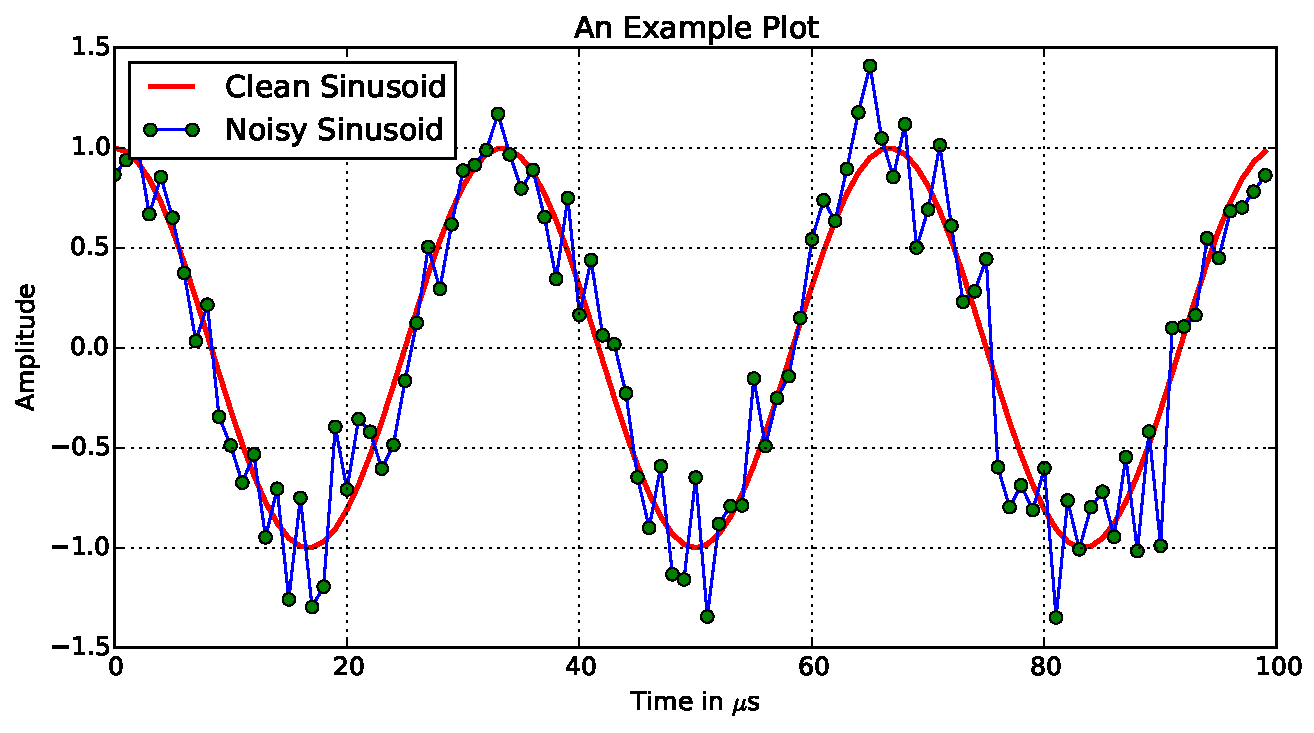
\includegraphics[width = 0.65\textwidth]{sinusoid.pdf}
\end{center}
\end{columns}
\end{frame}

\begin{frame}[fragile,allowframebreaks=0.8]
 {Another Example}
\begin{columns}
\column{0.4\textwidth}
\begin{itemize}
\item Even rather complicated graphics are easy to generate using Matplotlib.
\item The code for the attached diagram is shown in 
\url{https://github.com/mahehu/SGN-41007}.
\end{itemize}
\column{0.6\textwidth}

\begin{center}
	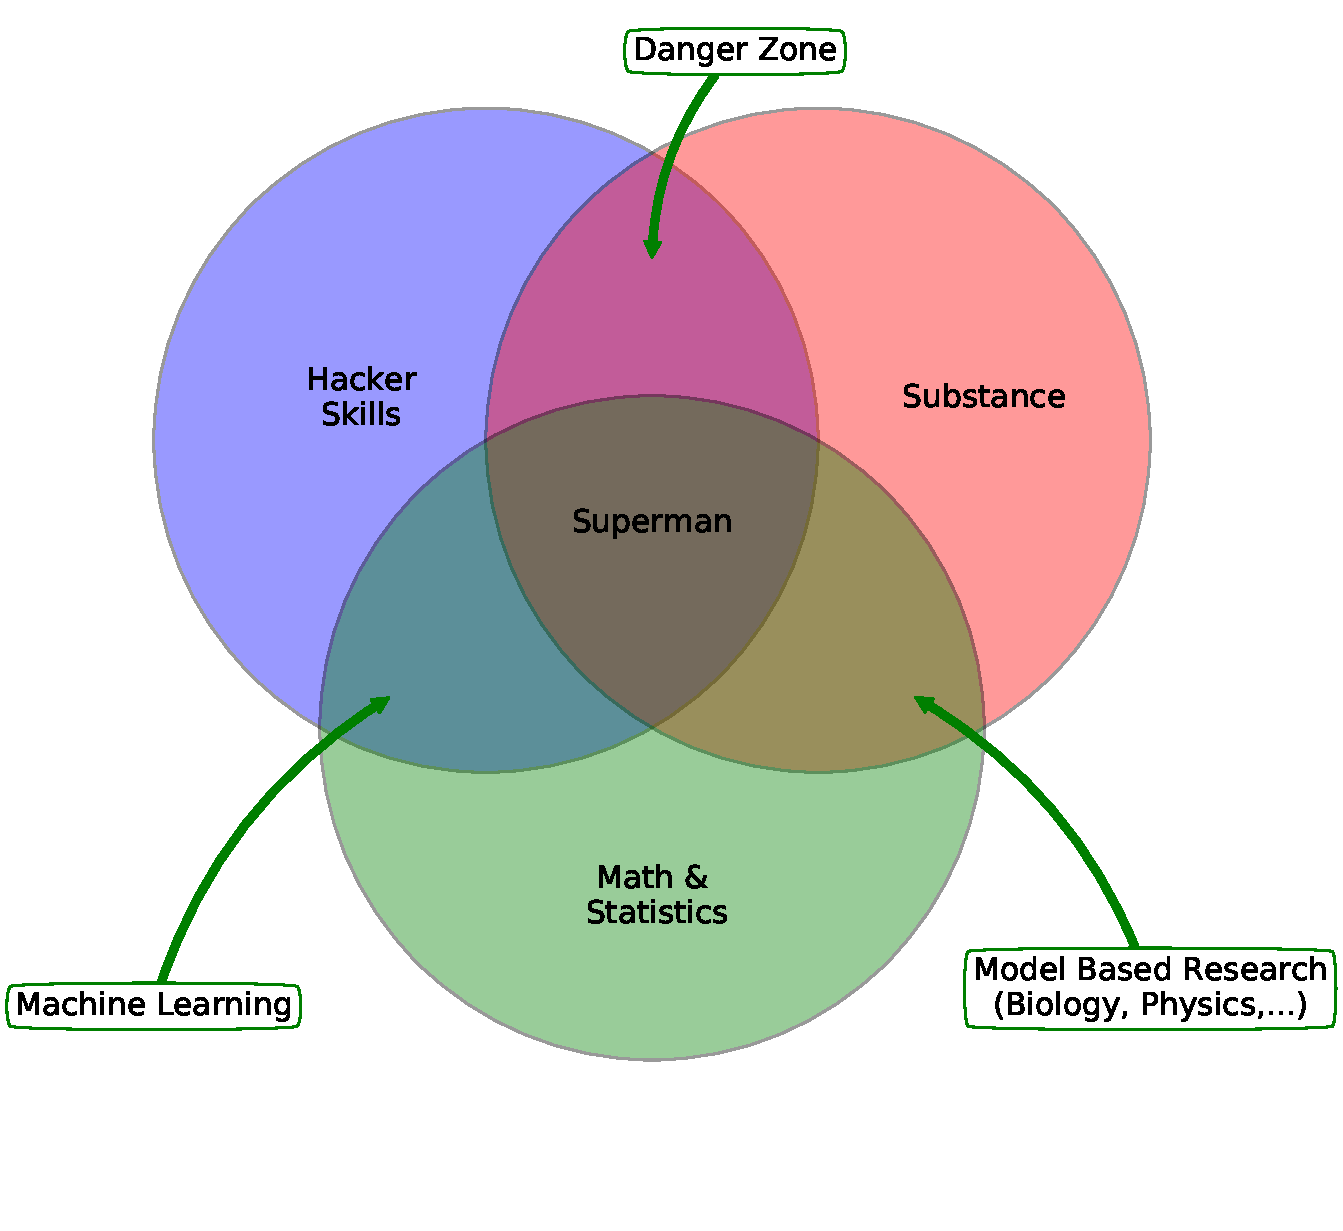
\includegraphics[width = \textwidth]{danger_zone.pdf}
\end{center}
\end{columns}
\end{frame}


\end{document}

